\documentclass[a4paper]{article}
\usepackage[utf8]{inputenc}
\usepackage[fleqn]{amsmath}
\usepackage{amssymb}
\usepackage{mathtools}
\usepackage{amsfonts}
\usepackage{lastpage}
\usepackage{tikz}
\usepackage{float}
\usepackage{textcomp}
\usetikzlibrary{patterns}
\usepackage{pdfpages}
\usepackage{gauss}
\usepackage{fancyvrb}
\usepackage[table]{colortbl}
\usepackage{fancyhdr}
\usepackage{graphicx}
\usepackage[margin=2.5 cm]{geometry}

\delimitershortfall-1sp
\newcommand\abs[1]{\left|#1\right|}

\definecolor{listinggray}{gray}{0.9}
\usepackage{listings}
\lstset{
	language=,
	literate=
		{æ}{{\ae}}1
		{ø}{{\o}}1
		{å}{{\aa}}1
		{Æ}{{\AE}}1
		{Ø}{{\O}}1
		{Å}{{\AA}}1,
	backgroundcolor=\color{listinggray},
	tabsize=2,
	rulecolor=,
	basicstyle=\scriptsize,
	upquote=true,
	aboveskip={0.2\baselineskip},
	columns=fixed,
	showstringspaces=false,
	extendedchars=true,
	breaklines=true,
	prebreak =\raisebox{0ex}[0ex][0ex]{\ensuremath{\hookleftarrow}},
	frame=single,
	showtabs=false,
	showspaces=false,
	showlines=true,
	showstringspaces=false,
	identifierstyle=\ttfamily,
	keywordstyle=\color[rgb]{0,0,1},
	commentstyle=\color[rgb]{0.133,0.545,0.133},
	stringstyle=\color[rgb]{0.627,0.126,0.941},
  moredelim=**[is][\color{blue}]{@}{@},
}
\newcommand{\comment}[1]{%
  \text{\phantom{(#1)}} \tag{#1}}
\lstdefinestyle{base}{
  emptylines=1,
  breaklines=true,
  basicstyle=\ttfamily\color{black},
}

\usepackage{tikz}
\tikzset{main node/.style={circle,fill=white!20,draw,minimum size=1cm,inner sep=0pt},}


\pagestyle{fancy}
\def\checkmark{\tikz\fill[scale=0.4](0,.35) -- (.25,0) -- (1,.7) -- (.25,.15) -- cycle;}
\newcommand*\circled[1]{\tikz[baseline=(char.base)]{
            \node[shape=circle,draw,inner sep=2pt] (char) {#1};}}
\newcommand*\squared[1]{%
  \tikz[baseline=(R.base)]\node[draw,rectangle,inner sep=0.5pt](R) {#1};\!}
\cfoot{Page \thepage\ of \pageref{LastPage}}
\DeclareGraphicsExtensions{.pdf,.png,.jpg}
\author{Ola Rønning (vdl761) \\ Tobias Hallundbæk Petersen (xtv657)}
\title{Advanced Computer Systems \\ Assignment 3}
\lhead{Advanced Computer Systems}
\rhead{Assignment 3}

\begin{document}
\maketitle
\section{Recovery Concepts}
\begin{enumerate}
\item If a system implements force and no-stealing, the system will not have to implement \texttt{REDO} nor \texttt{UNDO}. The system will not have to implement \texttt{REDO} as the state of system is always consistent on the non-volatile memory, this is because writes are forced to write to the the non-volatile memory. As the system does not implement stealing; non-volatile storage will never have dirty cells, and hence there will be nothing to \texttt{UNDO} after a crash.
\item The difference between non-volatile and stable storage, is that stable storage can recover from media failure by implementing redundancy. Both kind of storage can recover from crashes. The final kind of storage, volatile storage, can neither recover from media failure nor crashes.
\item The log tail is forced to stable storage, when either page is written to non-volatile storage or a transaction commits. The log tail is forced to stable storage before a page is written to ensure recoverability in case of a subsequent crash. The log tail must be forced to stable storage when a transaction is committed so that the updates performed by the transaction are recoverable in case of a crash. As volatile storage will not be recoverable from a crash, a log of system state represented by the the non-volatile storage after a crash is necessary. To ensure the durability of the system, it is therefore sufficient to maintain a log of system state represented by the storage that will survive a crash, i.e. non-volatile storage.
\end{enumerate}
\section{ARIES}\begin{table}[h!]
\begin{tabular*}{\textwidth}{@{\extracolsep{\fill}}lllll}
\texttt{LOG}&&&& \\
&&&&\\
\texttt{LSN} & \texttt{LAST\_LSN} & \texttt{TRAN\_ID} & \texttt{TYPE} & \texttt{PAGE\_ID} \\
\texttt{1} & \texttt{-} & \texttt{-} & \texttt{begin CKPT} & \texttt{-} \\
\texttt{2} & \texttt{-} & \texttt{-} & \texttt{end CKPT} & \texttt{-} \\
\texttt{3} & \texttt{NULL} & \texttt{T1} & \texttt{update} & \texttt{P2} \\
\texttt{4} & \texttt{3} &\texttt{T1} & \texttt{update} & \texttt{P1} \\
\texttt{5} & \texttt{NULL} & \texttt{T2} & \texttt{update} & \texttt{P5} \\
\texttt{6} & \texttt{NULL} & \texttt{T3} & \texttt{update} & \texttt{P3} \\
\texttt{7} & \texttt{6} & \texttt{T3} & \texttt{commit} & \texttt{-} \\
\texttt{8} & \texttt{5} & \texttt{T2} & \texttt{update} & \texttt{P5} \\
\texttt{9} & \texttt{8} & \texttt{T2} & \texttt{update} & \texttt{P3} \\
\texttt{10} & \texttt{6} & \texttt{T3} & \texttt{END} & \texttt{-} \\
\end{tabular*}
\caption{The log records before a crash.}
\label{log}
\end{table}
\subsection*{1.}
\begin{table}[h!]
\begin{tabular*}{\textwidth}{@{\extracolsep{\fill}}lllll}
\texttt{Transaction table}&&&& \\
&&&&\\
\texttt{TRAN\_ID} & \texttt{Status} & \texttt{last\_LSN} \\
\texttt{T1} & \texttt{progress} & \texttt{4} \\
\texttt{T2} & \texttt{progress} & \texttt{9} \\
\end{tabular*}
\caption{The transaction table after the crash, based on the log, see table~\ref{log}.}
\label{trans}
\end{table}
\begin{table}
\begin{tabular*}{\textwidth}{@{\extracolsep{\fill}}lllll}
\texttt{Dirty page table}&&&& \\
&&&&\\
\texttt{Page\_ID} & \texttt{recLSN} \\
\texttt{P1} & \texttt{4}\\
\texttt{P2} & \texttt{3}\\
\texttt{P3} & \texttt{6}\\
\texttt{P5} & \texttt{5}\\
\end{tabular*}
\caption{The dirty page table after the crash, based on the log, see table~\ref{log}.}
\label{dirty}
\end{table}
The transaction table, see table~\ref{trans}, is based on the log, see table~\ref{log}. Transaction three has ended and hence is not on the Transaction table, whilst transaction one and two are still in progress, when the crash occurs.\\
The dirty page table, see table~\ref{dirty}, is based on the log, see table~\ref{log}. The \texttt{recLSN} field represents the first log sequence number identifying a update dirtying a particular page. Pages one, two three and five was written to after the last checkpoint where the dirty page table was flushed.
\subsection*{2.}
The set of winner transaction are transactions that have committed and ended before the crash occurs, whilst the loser set represents the transactions that are still in progress. Hence the winner set for the log, see table~\ref{log}, is \{\texttt{T3}\} and the losers set is \{\texttt{T1}, \texttt{T2}\}.
\subsection*{3.}
The redo phase will begin at LSN three as this is the lowest LSN recorded in the dirty page table. The undo phase will end at LSN three, the highest LSN will be picked and after the modification it identifies is undone its \texttt{LAST\_LSN} will be added until all transaction recorded in the Transaction table have \texttt{NULL} recorded in their \texttt{LAST\_LSN} field.
\subsection*{4.}
The set of LSNs that identify log records may need to be rewritten are \{3, 4, 8, 9\}. Log record three may need to be rewritten as it is on the dirty page table, see table~\ref{dirty}, its LSN is equal to the recorded recLSN on the dirty table. Lastly we are using ARIES and transaction one has not been committed. Log records three, four, eight and nine are in the set by a similar argument.
\subsection*{5.}
The set of LSNs that identify log records that must be undone during the undo phase is \{9, 8, 5,4,3\}. These are the modification done by the loser transactions before the last checkpoint.
\subsection*{6.}
\begin{table}[H]
\begin{tabular*}{\textwidth}{@{\extracolsep{\fill}}lllll}
\texttt{LOG}&&&& \\
&&&&\\
\texttt{LSN} & \texttt{LAST\_LSN} & \texttt{TRAN\_ID} & \texttt{TYPE} & \texttt{PAGE\_ID} \\
\texttt{1} & \texttt{-} & \texttt{-} & \texttt{begin CKPT} & \texttt{-} \\
\texttt{2} & \texttt{-} & \texttt{-} & \texttt{end CKPT} & \texttt{-} \\
\texttt{3} & \texttt{NULL} & \texttt{T1} & \texttt{update} & \texttt{P2} \\
\texttt{4} & \texttt{3} &\texttt{T1} & \texttt{update} & \texttt{P1} \\
\texttt{5} & \texttt{NULL} & \texttt{T2} & \texttt{update} & \texttt{P5} \\
\texttt{6} & \texttt{NULL} & \texttt{T3} & \texttt{update} & \texttt{P3} \\
\texttt{7} & \texttt{6} & \texttt{T3} & \texttt{commit} & \texttt{-} \\
\texttt{8} & \texttt{5} & \texttt{T2} & \texttt{update} & \texttt{P5} \\
\texttt{9} & \texttt{8} & \texttt{T2} & \texttt{update} & \texttt{P3} \\
\texttt{10} & \texttt{6} & \texttt{T3} & \texttt{END} & \texttt{-} \\
\multicolumn{5}{c}{\texttt{CRASH, RESTART}}\\
\texttt{11} & \texttt{-} & \texttt{T2} & \texttt{CLR;undo LSN 9} & \texttt{P3} \\
\texttt{12} & \texttt{-} & \texttt{T2} & \texttt{CLR;undo LSN 8} & \texttt{P5} \\
\texttt{13} & \texttt{-} & \texttt{T2} & \texttt{CLR;undo LSN 5} & \texttt{P5} \\
\texttt{14} & \texttt{13} &\texttt{T2} & \texttt{END} & \texttt{-} \\
\texttt{15} & \texttt{-} & \texttt{T1} & \texttt{CLR;undo LSN 4} & \texttt{P1} \\
\texttt{16} & \texttt{-} & \texttt{T1} & \texttt{CLR;undo LSN 3} & \texttt{P2} \\
\texttt{17} & \texttt{16} & \texttt{T1} & \texttt{END} & \texttt{-} \\
\end{tabular*}
\caption{The log records until restart.}
\label{crs}
\end{table}
The table~\ref{crs} represents the log after recovery has been completed. Neither the analysis nor redo phase will write anything to the log. The redo phase could write end type record if there were any committed transactions that had not been ended, however, this is not the case. The undo phase will iterate over all loser transactions undoing the highest current LSN until the \texttt{LAST\_LSN} is \texttt{NULL} by which the transaction will be ended.
\section{Performance Measurements}
\begin{enumerate}
  \item The author and title of a generated book is a random alphanumeric string of a fixed length, configured upon construction. The default length of is ten characters. The ISBN is a random positive integer, between one and \(2^{32}-1\). Given that we are experimenting with upto twenty five workers, each performing five hundred units of work, the range of the ISBNs makes it effectively collision free. As we only interact with books that have the editors pick flag set, we set this by default. We always introduce one hundred copies of a book when at a price of a single unite. One hundred copies was chosen empirically as a balance between not having to many BookStoreInterations fail, and the FrequentStockManagerInteraction have something to do. The source code was compiled to JRE-1.7. The experiments were run on four core 2.5 GHz CPU, Intel Core i5-2400M, with 3.6 GiB of available DDR2 ram and a Intel Corporation 82579V Gigabit Network Connection. The measurements for the experiment were not repeated, and a total of five measurements were taken. We ranged from two to twenty four threads. The limited range were do to the high time consumption associated with communicating over the network. After the data was taken, we normalized it, such that the development of both curves were visible. This was necessary as there were large difference in both latency and throughput between the online and offline benchmark. The data manipulation to construct the desired plots were performed in python.
  \item Figure \ref{goodput} and \ref{latency} show the goodput and latency benchmarks respectively. The plots show the curves for the executions in the same address space, called offline, and one for executions across address spaces, called online. We can see the goodput is rising in the offline version whereas it is falling drastically in the online version, this is due to the fact that the online version in the current handout cannot handle concurrent requests, whereas the offline version handles this fine. Which is why we see an increasing goodput the more concurrent requests we get in the offline version. The latency of the two seem to both follow an exponential function, where the online has a much higher factor. You would expect the latency of the online version to be much higher than that of the offline, as there is a smaller overhead when doing executionins in the same address space, compared to the same across address spaces.
    \begin{figure}[H]
      \center
      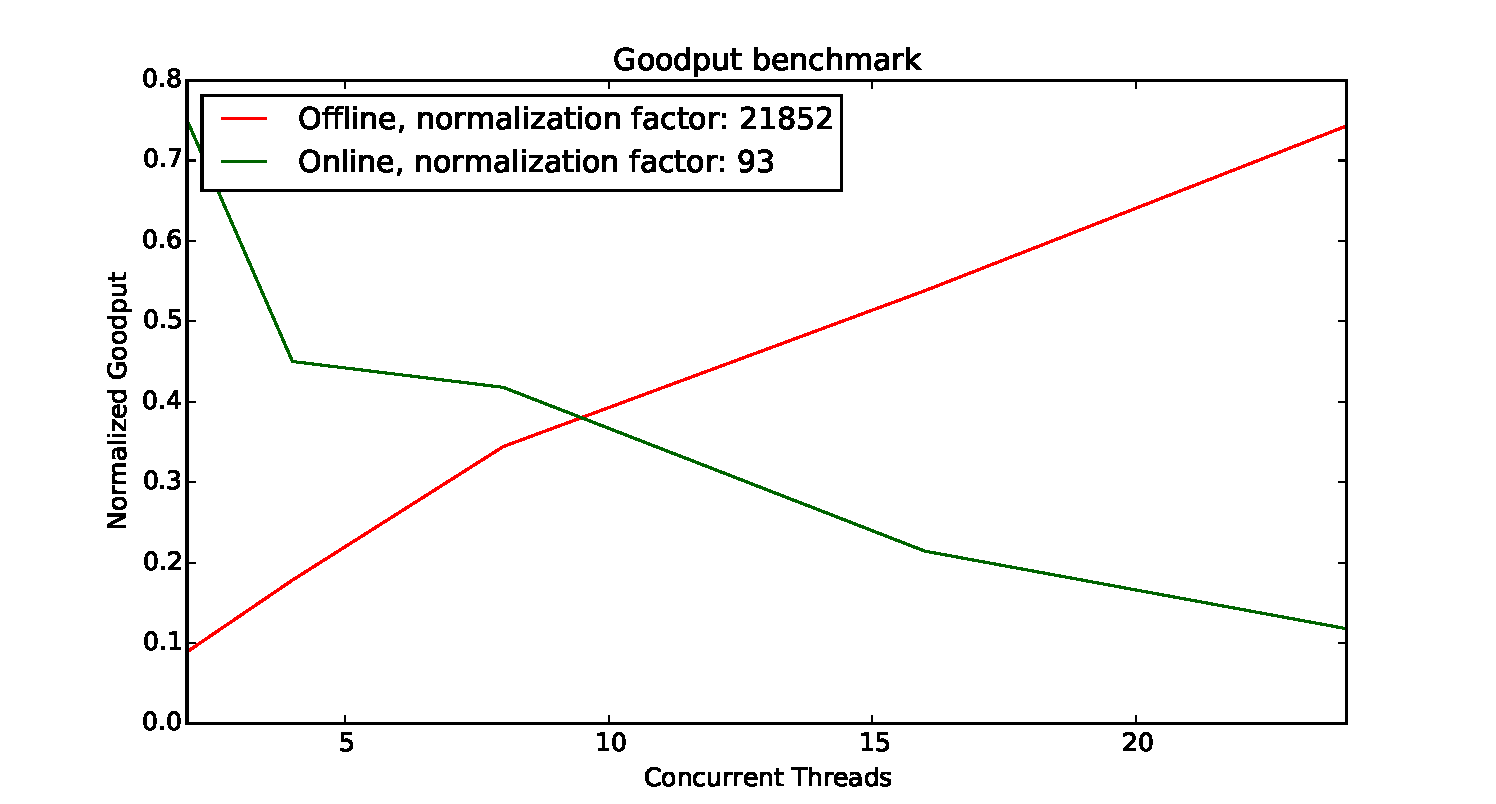
\includegraphics[width=0.7\textwidth]{./goodput.pdf}
      \caption{The goodput benchmark of the online and offline version of acertainbookstore. The data has been normalized.}
      \label{goodput}
    \end{figure}
    \begin{figure}[H]
      \center
      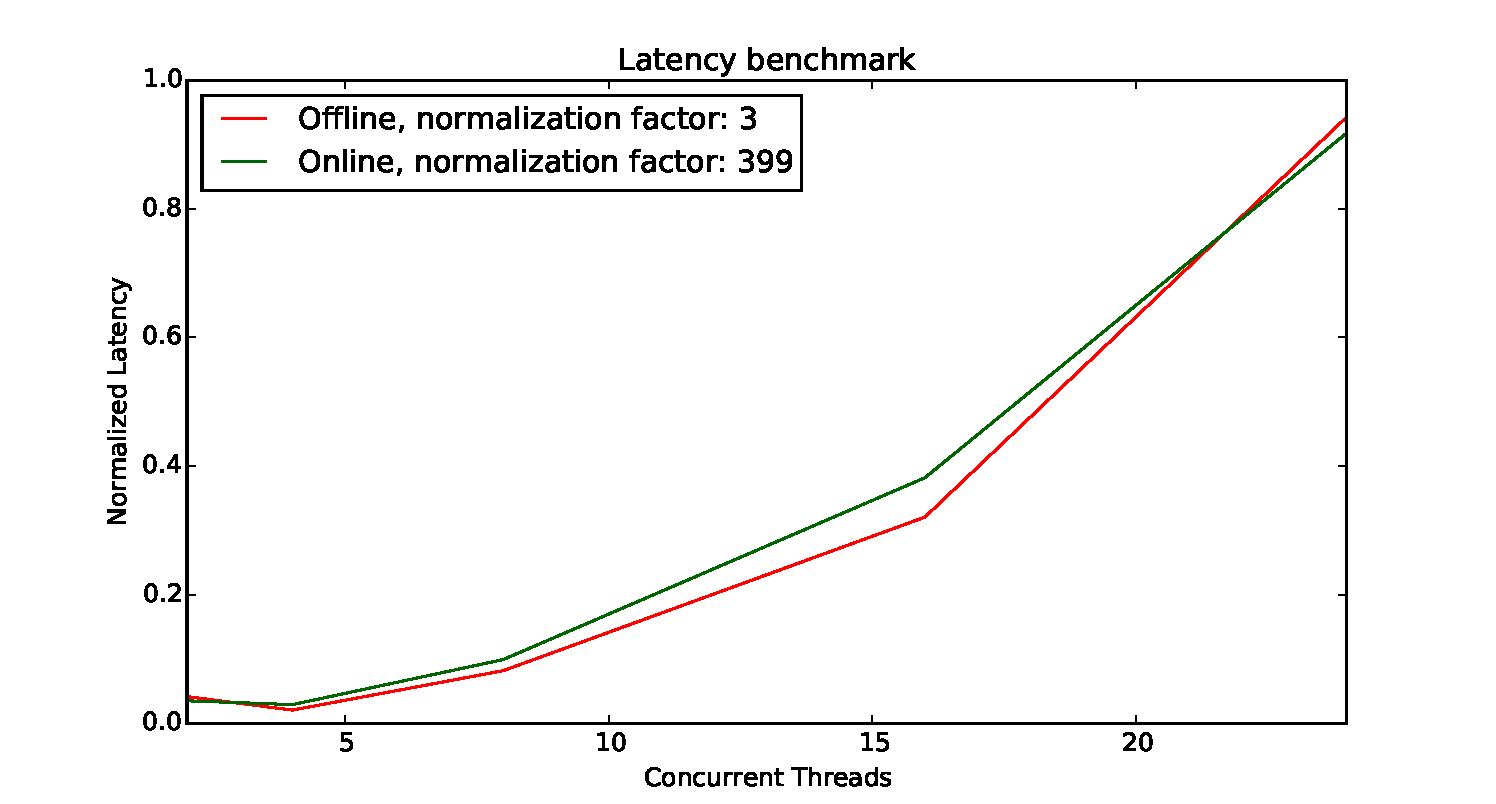
\includegraphics[width=0.7\textwidth]{./latency.pdf}
      \caption{The latency benchmark of the online and offline version of acertainbookstore. The data has been normalized.}
      \label{latency}
    \end{figure}
  \item The workloads seem reliable to predict the performance of the bookstore, but it depends on whether or not the division of labour corresponds with that of actual execution. The latency and goodput are two metrics worth measuring when benchmarking the system, as these metrics are highly in focus when designing such a system. Another metric to measure would be the overhead of the two versions of the system, this is going to correlate with the latency, but to which degree could be interesting.
\end{enumerate}
\end{document}